\documentclass[
reprint,amsmath,amssymb,showpacs,citeautoscript,prb,twocolumn,notitlepage,floatfix
]{revtex4-1}

\usepackage{graphicx}% Include figure files
\usepackage{bm}% bold math
\usepackage{float}
\usepackage{epstopdf}
\usepackage{tikz}
\usepackage{setspace}
\usepackage{physics}
% \usepackage{lipsum}
% \usepackage{babel}

\begin{document}

\preprint{APS/123-QED}

\title{Title 2: Electric Boogaloo}

\author{Evan Bluhm}
 
\noaffiliation
\date{\today}

% \begin{abstract}

% \end{abstract}

\maketitle
\setstretch{1.5}



% \begin{figure}[ht]
%     \begin{center}
%         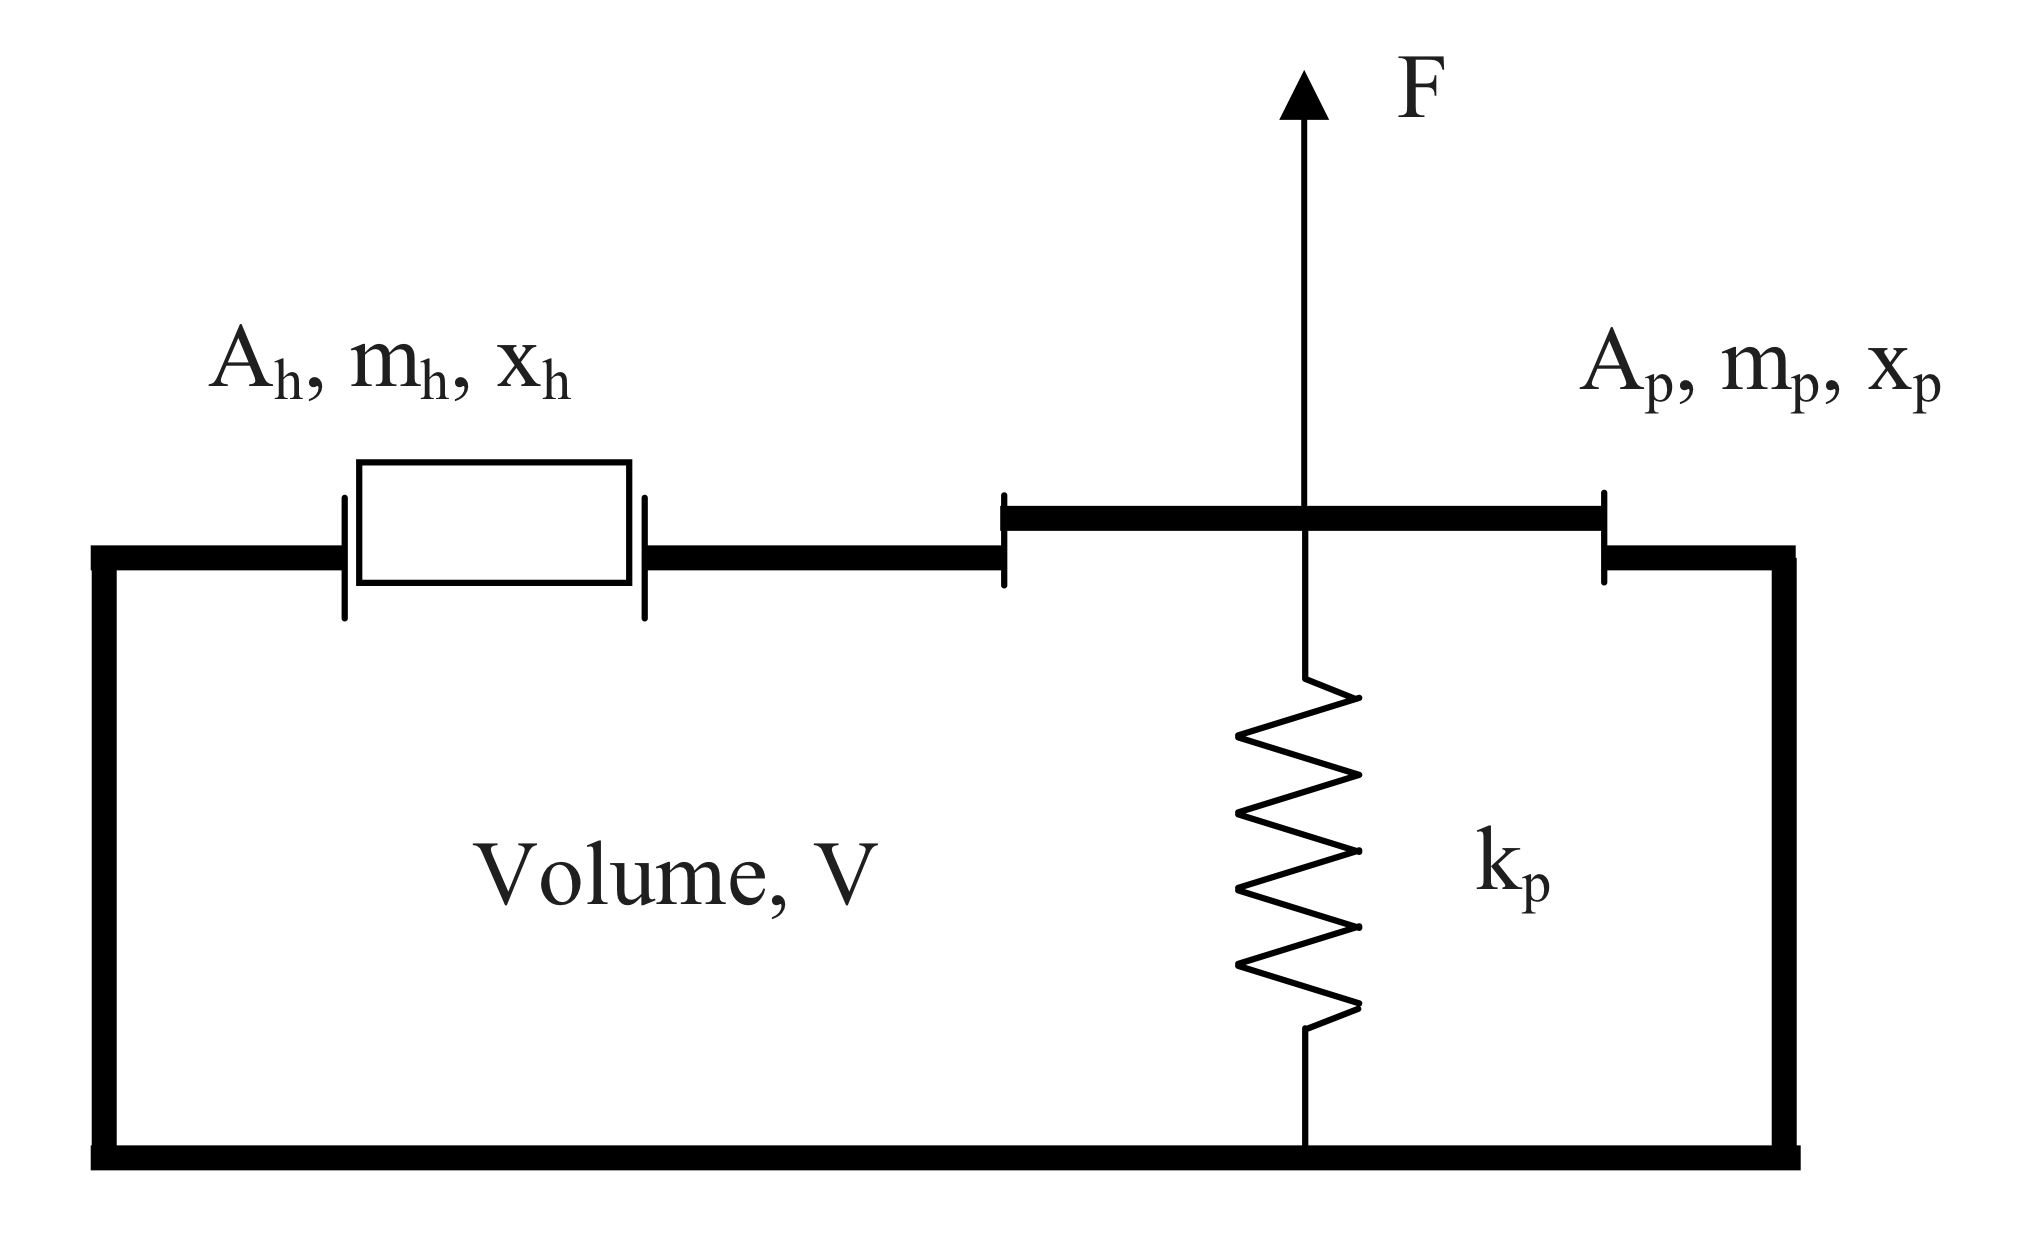
\includegraphics[width=0.4\textwidth]{images/french2008-two-mass-model.png}
%         \caption{Two-mass model of the low-frequency behavior of the guitar. The soundboard and guitar cavity are replaced by coupled oscillators.  Reprinted from  French, R. (2008). Engineering the Guitar: Theory and Practice. Springer US.}
%         \label{fig:two-mass-model}
%     \end{center}
% \end{figure}

\setstretch{1.0}
\nocite{*}
\bibliographystyle{apalike}
\bibliography{paper}% Produces the bibliography via BibTeX.

\end{document}
%
% ****** End of file apssamp.tex ******
